		\begin{enumerate}
			\item \begin{enumerate}
				\item \phantom{x}
				
				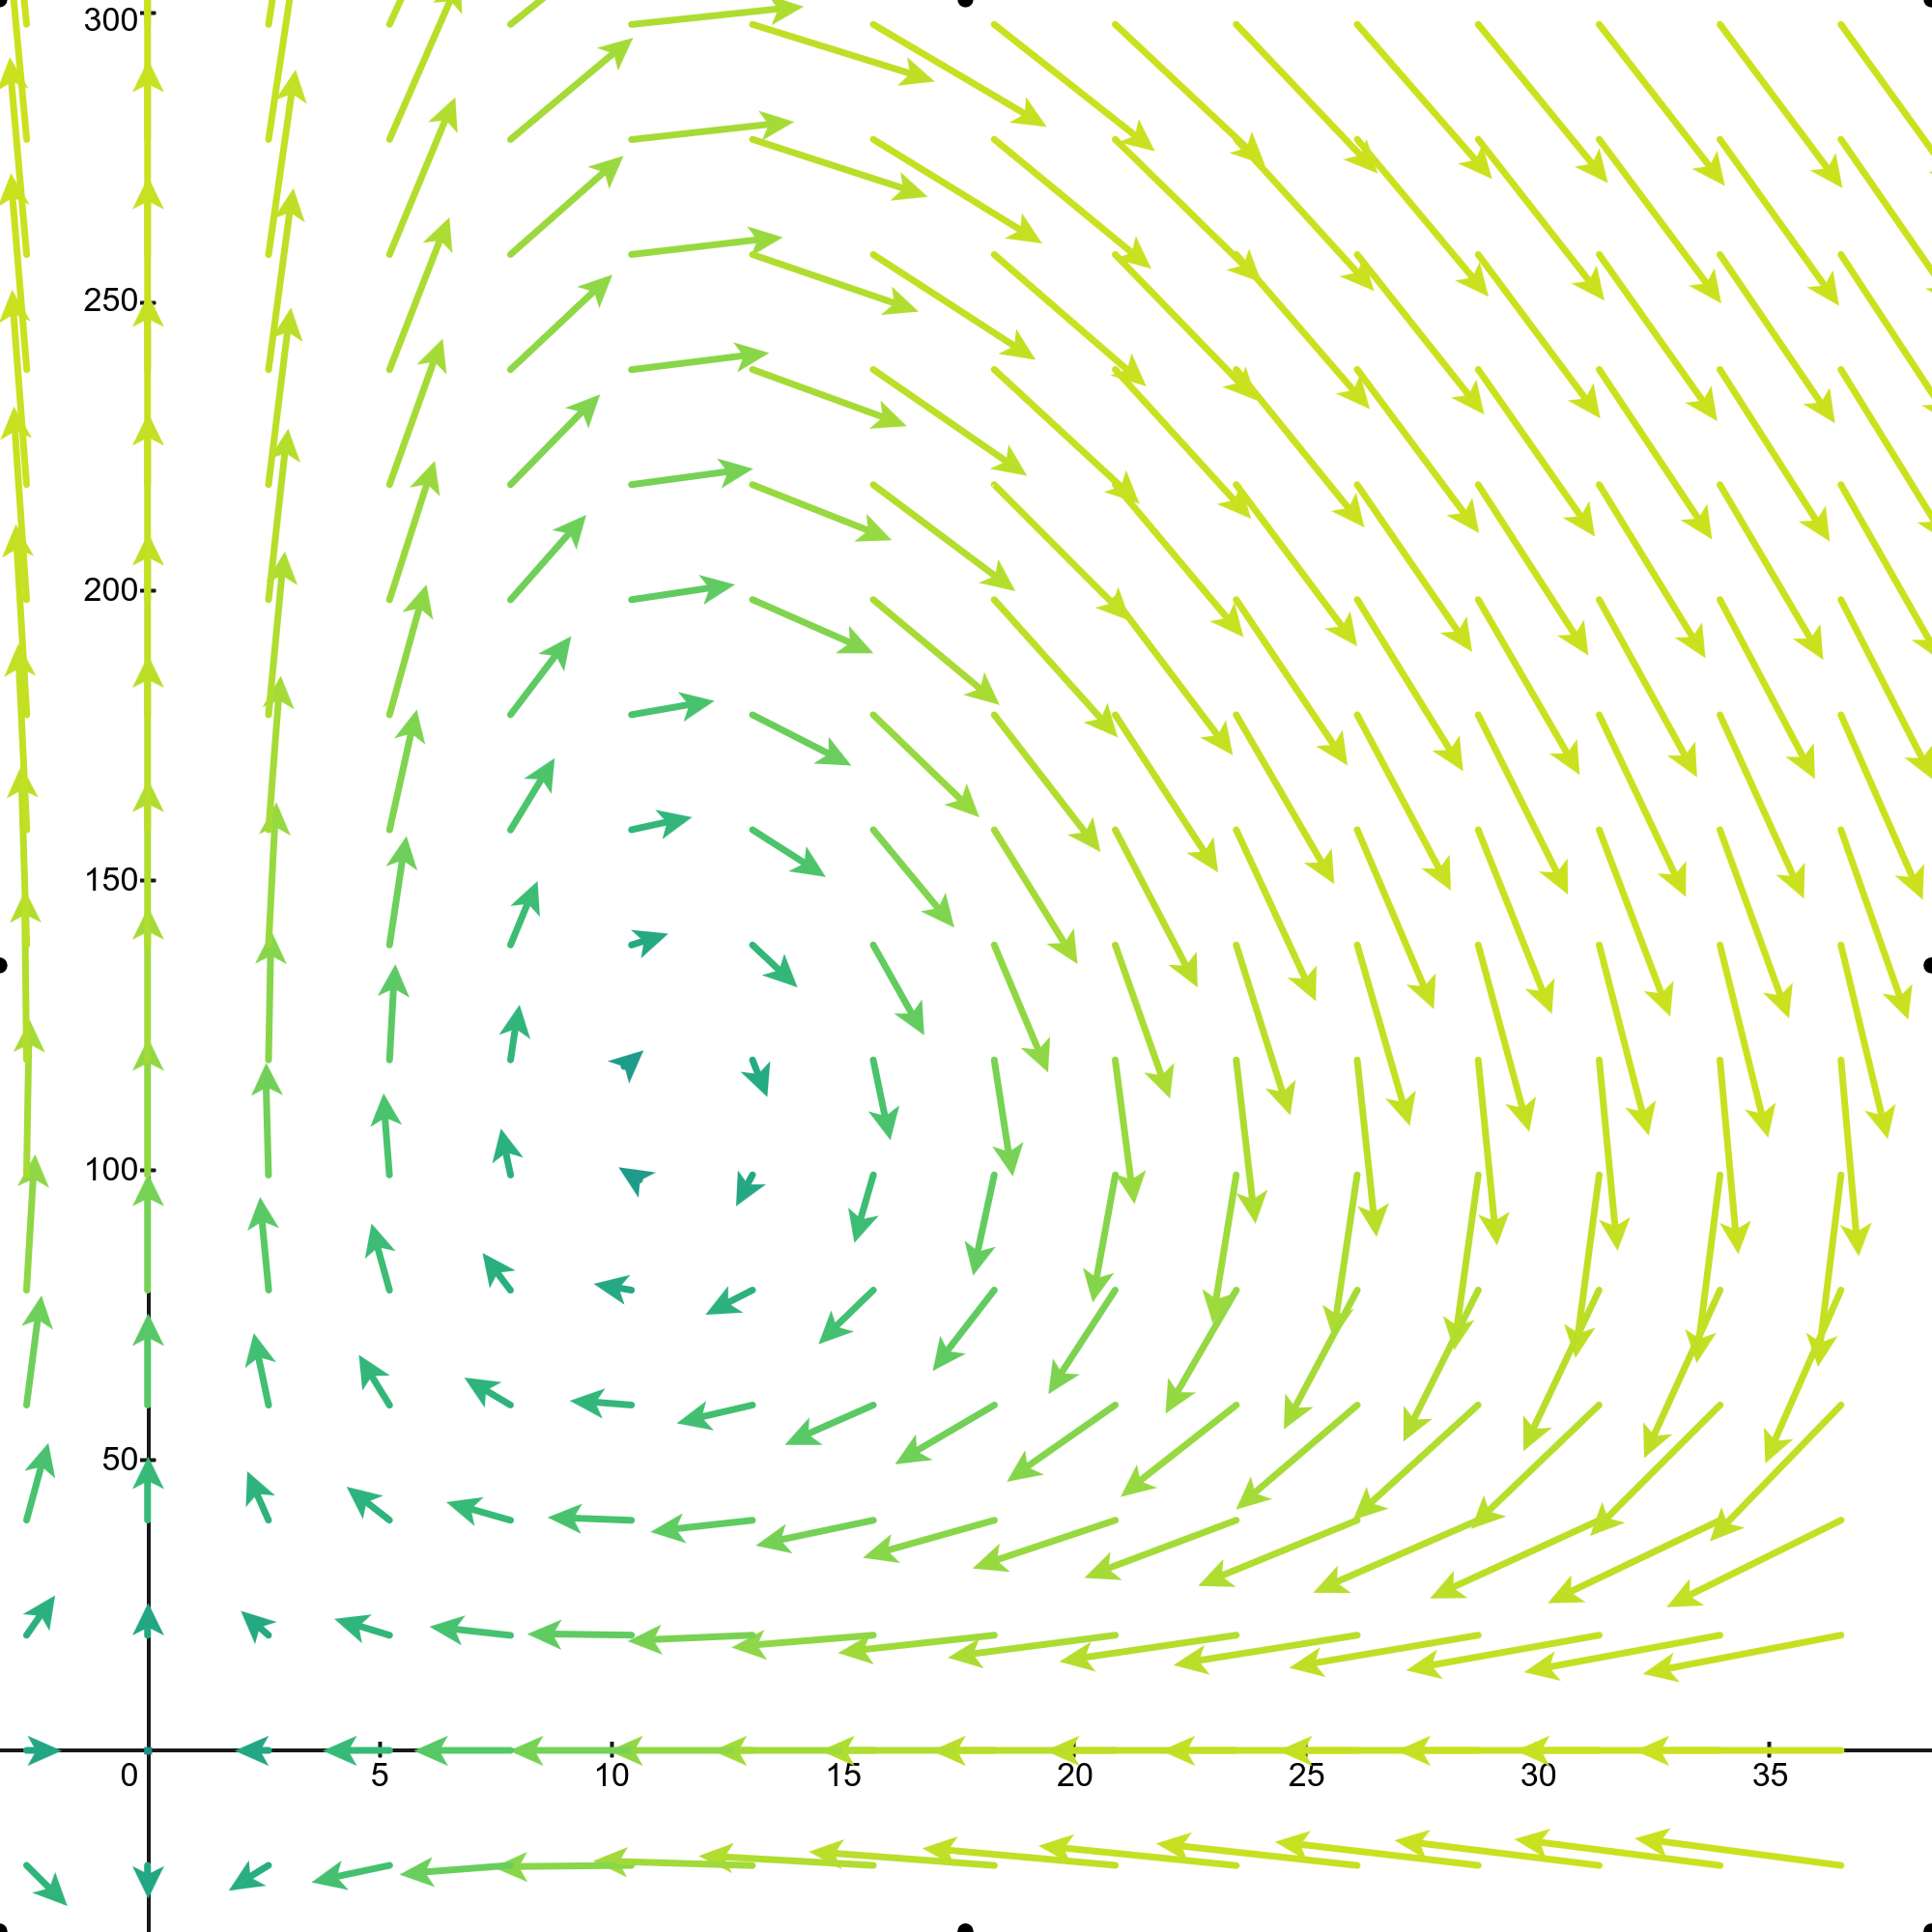
\includegraphics[width=3in]{resources/tutorial-02-1a.png}

				\item Arrows to the right of $F=11$ point down. That means as there are more foxes, the rabbit population decreases.
				Arrows to the left of $F=11$ point up, so as there are fewer foxes, there are more rabbits. If the arrows were oriented in the opposite direction,
				more foxes would lead to more rabbits, which is the opposite of what we would expect if the foxes ate the rabbits.
			\end{enumerate}
			\item \begin{enumerate}
				\item As long as $a,b,c,d>0$, there will be periodic behaviour.
				However, if any of the parameters becomes zero, the behaviour will change.
				\item 
				\item If we leave $a,c,d$ as they are and set $b$ to zero, the foxes will never die.
				Thus, the fox population will grow and grow as long as there are rabbits available. However,
				once the foxes eat the rabbits to extinction, they fox population will be unchanged, since the foxes are
				immortal!
			\end{enumerate}
			\item \begin{enumerate}
				\item We know that a maximum rabbit population occurs when $R'=0$. Manipulating the equation for
				$R'$, we find that $R'=0$ when $F=c/d$.
				\item Manipulating the equation for $F'$, we find that $F'=0$ when $R=b/a$.
				\item If neither populations change, then we must have $F'=0$ and $R'=0$. This occurs when
				$(F,R)=(c/d, b/a)$ or $(F,R)=(0,0)$.
				\item If we allow $d$ or $a$ to be zero, the derivations we did in the previous parts
				are no longer valid (we can't divide by zero)! If $c$ or $d$ equals zero, then there are equilibrium solutions
				where one population is positive and the other zero. Since populations cannot be negative, this prevents
				periodic behaviour. So, our analysis here helps explain part \ref{qual}.
			\end{enumerate}
		\end{enumerate}
